\documentclass[text.tex]{subfiles}

\begin{document}

\section{Quasicrystal}\label{sec_quasicrystalEaseIn}%---------------------------------------------------
In two dimensions a quasicrystal can be viewed as a subset of complex numbers $\Lambda\subset\CC$ following these five properties:

\begin{enumerate}
\item rotational symmetry: $$\exists\,\zeta = e^{2\pi i/n}:\; \zeta\Lambda = \Lambda$$
\item dilation: $$\exists\,\beta\in\RR\setminus\{-1,1\}:\; \beta\Lambda\subset \Lambda$$
\item uniform discreteness: $$\exists\,r_1>0,\; \forall z_1,z_2\in\Lambda, z_1\neq z_2:\; |z_1-z_2|>r_1$$
\item relative density: $$\exists\,r_2>0,\; \forall z\in\CC:\; B(z,r_2)\cap\Lambda \neq \emptyset$$
\item finite local complexity: $$\forall\,\rho>0:\;\big|\{\Lambda\cap B(x,\rho)\;|\;\forall x\in\Lambda\}\big| < \infty$$
\end{enumerate}

\begin{remark}
Properties 3. and 4. together make quasicrystal to be a Delone set.
\end{remark}

It stems form these properties alone, that among other constants a quasicrystal is linked to a root of unity $\zeta$ and to a number $\beta\in\RR\setminus\{-1,1\}$. Of course not every pair $(\zeta, \beta)$ is associated with a quasicrystal.

In the next section we will go through which numbers are associated with a quasicrystal and where do they come from. 

\section{Pisot-cyclotomic numbers}\label{sec_pisotCyclotomic}%--------------------------------------------------------
Pisot-cyclotomic numbers are Pisot and are algebraically related to roots of unity. We will use these numbers in place of $\beta$ from previous section. 

\begin{definition}\label{def_pisotCyclotomic}
Let $\rho = 2\cos\left(2\pi/n\right)$ for a given $n>4$, its extension ring $\ZZ[\rho]$ and $m$ order of $\rho$. A \textbf{Pisot-cyclotomic} number of degree $m$, of order $n$ associated to $\rho$ is a Pisot number $\beta \in \ZZ[\rho]$ such that
$$\ring = \ZZ[\rho]$$
\end{definition}

Nontrivial $n$th root of unity $\zeta = e^{2\pi i/n}$ is by definition a solution to equation
$$\frac{\zeta^n-1}{\zeta-1} = \zeta^{n-1}+\zeta^{n-2}+\dots+\zeta+1 = 0$$
further for $\rho = 2\cos\left(2\pi/n\right)$ it holds
$$\rho = \zeta + \bar{\zeta}\quad\Rightarrow\quad \zeta^2 = \rho\zeta - 1$$
Therefore for extension rings $\ZZ[\zeta]$ and $\ZZ[\rho]$ we have
$$\ZZ[\zeta] = \ZZ[\rho] + \ZZ[\rho]\zeta$$
and finally for Pisot-cyclotomic $\beta$ associated to $\rho$ we acquire
$$\ZZ[\zeta] = \ring + \ring\zeta$$
Such countable ring is of course $n$-fold rotationally invariant
$$\zeta^k\ZZ[\zeta] \subset \ZZ[\zeta]\qquad k\in\widehat{n-1}$$

To summarize $\beta$ is real and a Pisot and it can be used to decompose $n$-fold rotationally invariant complex ring $\ZZ[\zeta]$ as $\ring + \ring\zeta$. 

For further work we will need actual values of Pisot-cyclotomic numbers and so in the next section we will show a method for finding quadratic Pisot-cyclotomic numbers, whose quasicrystals we will later analyze. The method could of course be generalized to different degrees. 

\subsection{Quadratic Pisot-cyclotomic numbers}
As stated in preliminaries, the degree of root of unity of order $n$ is $\varphi(n)$ (where $\varphi$ is the Euler's function). From the decomposition in the previous section we can easily infer that the degree of $\zeta$ is double of degree of $\beta$ (or $\rho$). Moreover we are looking for $\beta$ of degree $2$. Together we acquire following equation. 
$$\varphi(n) = 2\cdot 2 = 4$$
With help from the Euler's product formula we can show that such equation holds only for $n\in\{5,8,10,12\}$. 

For each $n\in\{5,8,10,12\}$ there is $\rho = 2\cos\left(2\pi/n\right)$ and for each such $\rho$ there are $\beta \in \ZZ[\rho]$ following the definition \ref{def_pisotCyclotomic}. 

To summarize, quadratic Pisot-cyclotomic numbers $\beta$ can only be associated to quasicrystals with $5$-fold, $8$-fold or $12$-fold rotational symmetries. Even though we are mainly focusing on two dimensional quasicrystals, that is not dictated by the quadratic-ness of $\beta$. Quadratic Pisot-cyclotomic numbers are also associated to arbitrarily dimensional quasicrystals. For example we will also study one dimensional quasicrystals. 

We close this section with a list of quadratic Pisot-cyclotomic numbers (table \ref{tab_quadraticPisotCyclotomic}). 

\begin{table}[h!]
\centering
\begin{tabular}{cccc}
$n$ & $\rho$ & $\beta$ & $\zeta$ \\
\hline
$5$   & $2 \cos\left(\frac{2\pi}{5}\right)$   & $\frac{1+\sqrt{5}}{2} $   & $e^{2i\pi/5}$ \\
$8$   & $2 \cos\left(\frac{2\pi}{8}\right)$   & $ 1+\sqrt{2} $            & $e^{2i\pi/8}$ \\
$12$  & $2 \cos\left(\frac{2\pi}{12}\right)$  & $ 2+\sqrt{3} $            & $e^{2i\pi/12}$ \\
\end{tabular}
\caption{Pisot-cyclotomic numbers of degree $2$, of order $n$, associated to $\rho$.}
\label{tab_quadraticPisotCyclotomic}
\end{table}

\section{Quasicrystal model}%--------------------------------------------------------------------------------
There certainly are many ways to acquire a set that follows the properties listed in section \ref{sec_quasicrystalEaseIn}. We utilize the cut-and-project scheme described in section \ref{sec_cutAndProject}. 

The cut-and-project scheme requires among others crystallographic lattice $L$, the sets $V_1$ and $V_2$, and suitable projections $\pi_1$ and $\pi_2$ or $\ast$. Finding these is outside of scope of this work. For now we will continue using general notation with the promise of specifying these sets and projections once necessary. 

\begin{definition}\label{def_quasicrystal}
Let $\beta$ be a Pisot-cyclotomic number of order $n$, associated to $\rho = 2\cos\left(2\pi/n\right)$ (and $\zeta = e^{2\pi i/n}$). 

Further let $M,\, N\subset \RR^d$ and projection $\ast:M\rightarrow N$ follow the conditions of the cut-and-project scheme.

Lastly let $\Omega\subset N$ be bounded with nonempty interior. 

Then \textbf{$d$ dimensional quasicrystal linked to irrationality $\beta$ and window $\Omega$} is the set:
$$\quasi{\Omega} = \{ x \in M\; |\; x^\ast\in \Omega\}$$
\end{definition}

So far the entire theses was purely abstract. To give you an example of what quasicrystal might look like, there is the image \ref{fig_quasicrystalFirstExample} which shows finite sections of a two dimensional quasicrystal with $8$-fold rotational symmetry.

\begin{figure}[h]
\centering
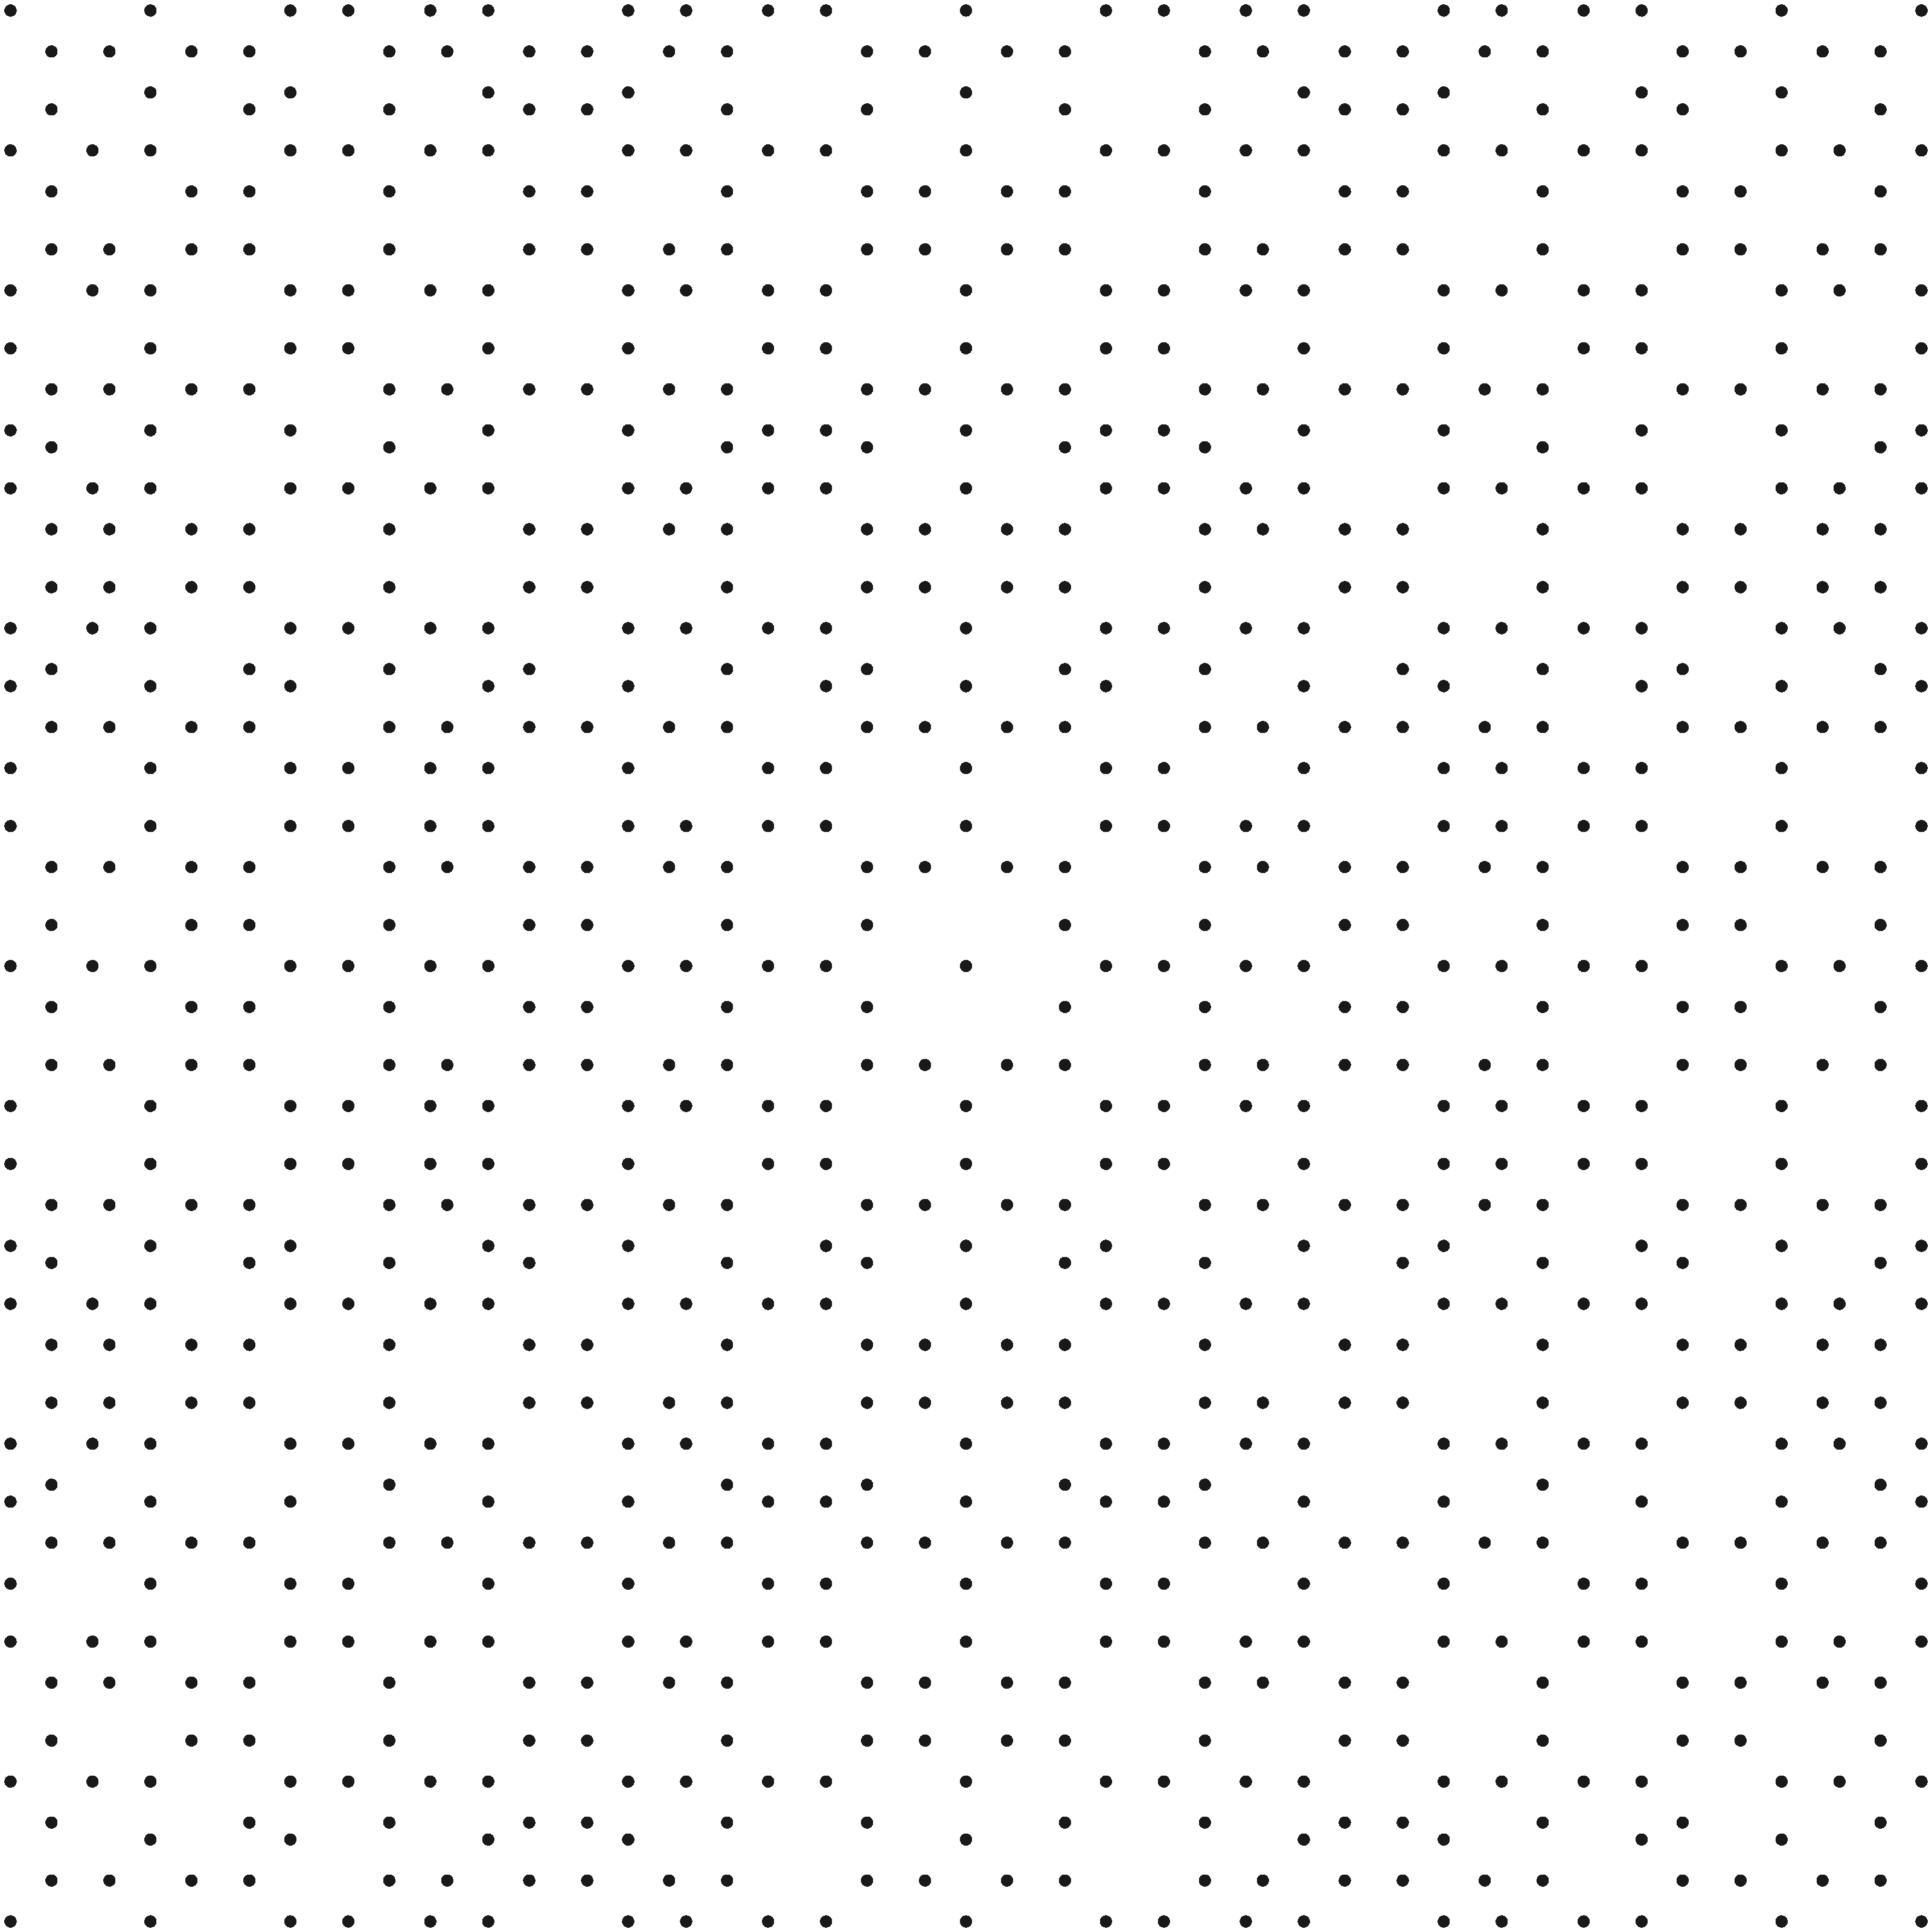
\includegraphics[width=0.9\textwidth]{img/firstExample}
\caption{Example of a two dimensional quasicrystal.}
\label{fig_quasicrystalFirstExample}
\end{figure}

To validate our quasicrystal model we of course have to show that it follows the properties in section \ref{sec_quasicrystalEaseIn}. However first we list few properties of our model which will help us show that. 

Since such general approach won't be necessary for our work, from now on we limit our scope to only quadratic Pisot-cyclotomic numbers (that greatly simplifies the scaling property). 

\begin{itemize}
\item Inclusion property: $$\Omega_1\subset\Omega_2 \quad\Rightarrow\quad \quasi{\Omega_1}\subset\quasi{\Omega_2}$$
\item Union property: $$\quasi{\Omega_1\cup\Omega_2} \,=\, \quasi{\Omega_1}\cup\quasi{\Omega_2}$$
\item Translation property: $$\quasi{\Omega+x^\ast} \quad=\quad \quasi{\Omega}+x\qquad \text{for}\; x\in M$$
\item Scaling property: $$\quasi{\beta\Omega} = \beta'\quasi{\Omega}$$
\end{itemize}

And now to validate our model. 

\begin{enumerate}
\item rotational symmetry: $$\exists\,\zeta = e^{2\pi i/n}:\; \zeta\Lambda = \Lambda$$
Rotational symmetry appears in quasicrystal if the window $\Omega$ has the same rotational symmetry.
\item dilation: $$\exists\,b\in\RR\setminus\{-1,1\}:\; b\Lambda\subset \Lambda$$
Using the scaling property and the inclusion property:
$$\beta\quasi{\Omega} = \quasi{\beta'\Omega} \subset \quasi{\Omega}$$
\item uniform discreteness: $$\exists\,r_1>0,\; \forall z_1,z_2\in\Lambda, z_1\neq z_2:\; |z_1-z_2|>r_1$$
\item relative density: $$\exists\,r_2>0,\; \forall z\in\CC:\; B(z,r_2)\cap\Lambda \neq \emptyset$$
The result of cut-and-project scheme is a Delone set if the window $\Omega$ is bounded with nonempty interior. 
\item finite local complexity: $$\forall\,\rho>0:\;\big|\{\Lambda\cap B(x,\rho)\;|\;\forall x\in\Lambda\}\big| < \infty$$
It has been shown that our model has even this property, however since this work explores this finite complexity it essentially proves this property as well. 
\end{enumerate}

Having quasicrystal defined and  our model validated, we will present our plan for the analysis. 

\section{General quasicrystal analysis}
In this section we will outline general method of analysis of any quasicrystal. Later we will use this method to analyze two dimensional and one dimensional quasicrystals. 

Analysis should reveal the structure of the points of the quasicrystal, for us that means listing all Voronoi tiles that appear in the qusicrystal's Voronoi diagram. 

To acquire such list we follow these steps: 
\begin{enumerate}
\item \textbf{Acquire arbitrary finite section of the quasicrystal}

In other words this means creating algorithm that for finite section $P\subset\RR^d$ returns $P\cap\quasi{\Omega}$. 
\item \textbf{Estimate covering radius of the quasicrystal $R_C$}

We are specifically interested in the upper bound $\hat{R}_C$ of the covering radius. 
\item \textbf{Generate superset of all finite sections spanning $B(2\hat{R}_C)$}

Each of these finite sections represents one Voronoi tile that appears in the quasicrystal's voronoi diagram. 
\item \textbf{Filter the superset to the final list of Voronoi tiles}
\end{enumerate}

These steps are general enough to analyze any quasicrystal associated with any Pisot-cyclotomic number and in any dimension. Unfortunately they are also too general and need to be specified for a specific quasicrystal. 

We close this chapter and our general overview of quasicrystals with discussion of window shapes. It is obviously impossible to analyze quasicrystal for arbitrary bounded $\Omega\subset N$ with nonempty interior. There however is a way to limit our scope to few window shapes that in some way represent all possible windows. 

\subsection{Analyzed window shapes}
We will use the properties of quasicrystals to gradually limit the set of analyzed windows. We start with all of the windows: 
$$\big\{\Omega\,|\, \Omega\subset N ,\;\text{bounded with nonempty interior}\big\}$$

Thanks to the union property we can limit our scope to a continuous convex bounded windows with nonempty interior since most more complicated windows are unions of continuous convex bounded window with nonempty interior: 
$$\big\{\Omega\,|\, \Omega\subset N ,\;\text{continuous convex bounded with nonempty interior}\big\}$$

Further thanks to the translation property we can limit our scope to a continuous convex bounded windows with nonempty interior centered around the origin: 
$$\big\{\Omega-\overline{\Omega}\,|\, \Omega\subset N ,\;\text{continuous convex bounded with nonempty interior}\big\}$$
where $\overline{\Omega}$ is the arithmetic mean (or "center of mass") of the window $\Omega$. 

Lastly thanks to the scaling property we can limit our scope to a continuous convex bounded windows with nonempty interior centered around the origin of diameter in $(1/\beta,1]$:
$$\big\{\Omega-\overline{\Omega}\,|\, \Omega\subset N ,\; d(\Omega)\in (1/\beta,1] ,\;\text{continuous convex bounded with nonempty interior}\big\}$$
where $d(\Omega)$ is the set diameter $d(\Omega) = \sup\{d(x,y)\,|\,x,y\in\Omega\}$

\begin{remark}
We could of course also pick any other $\beta$ multiple of $(1/\beta,1]$. 
\end{remark}

Of course even after all this limiting, the set of windows is still infinite. Therefore we will further limit our scope to three basic window shapes: rhombus, regular $n$-gon and a circle. The rhombus is not really a valid window since it is not sufficiently rotationally symmetrical, it is however fundamental to our method, more on this later. The regular $n$-gon represents the simplest window with sufficient rotational symmetry and the circle interesting for its circular symmetry. 

To summarize we will analyze quasicrystals for windows in shape of rhombus, regular $n$-gon and a circle centered around the origin of diameter in $(1/\beta,1]$. Technically there is an infinite amount of these windows as well however as we will see later it is already manageable. 

Finally we need to discuss the boundaries of the windows. Generally we will assume open windows i. e. we will exclude the boundary. The exception is the rhombus (and its one dimensional equivalent -- interval) for reasons we will also explain later. 

Now we have quasicrystal defined, model explored and windows limited. In the next chapter we will finally start the analysis. 


\end{document}
